\documentclass[aspectratio=169,final]{beamer}
\setbeamersize{text margin left=5pt,text margin right=5pt}
\setbeamertemplate{navigation symbols}{}


\usepackage{booktabs}
\usepackage{multirow}
\usepackage{tikz}

\usepackage{amsmath}
\newcommand{\expect}{\mathds{E}} %{{\rm I\kern-.3em E}}
\newcommand{\probability}{\mathds{P}} %{{\rm I\kern-.3em P}}
\newcommand{\indicator}{\mathds{1}} %{{\rm I\kern-.3em P}}
\DeclareMathOperator*{\argmax}{arg\,max} % thin space, limits underneath in displays
\DeclareMathOperator*{\argmin}{arg\,min} % thin space, limits underneath in displays

\begin{document}

\begin{frame}{\centering  Learning to Infer Graphics Programs from Hand-Drawn Images\\
    \centering\small  Kevin Ellis$^1$, Daniel Ritchie$^2$, Armando Solar-Lezama$^1$, Joshua B. Tenenbaum$^1$\\
  \small   $^1$: MIT. $^2$: Brown University.}
\centering
  \begin{tabular}{lllll}
\visible<2->{    \includegraphics[height = 0.1\textwidth]{figures/staircase}}&
\visible<3->{    \includegraphics[height = 0.1\textwidth]{figures/tree}}&
\visible<4->{    \includegraphics[height = 0.1\textwidth]{figures/gears}}&
\visible<5->{    \includegraphics[height = 0.1\textwidth]{figures/Simmons}&
        \includegraphics[height = 0.1\textwidth]{figures/randomFields}}
  \end{tabular}

  \vspace{.1cm}

\visible<6->{    \includegraphics[width = 0.9\textwidth]{firstSpotlightExample.pdf}}
  

  \end{frame}

\begin{frame}{Image$\to$Program Pipeline}
\centering  \includegraphics[width = 0.76\textwidth]{pipeline.pdf}

\vspace{1cm}

  \includegraphics[width = 0.7\textwidth]{exampleProgramsSpotlight.pdf}
\end{frame}


\begin{frame}{Parsing images into \LaTeX~TikZ Commands}

  %% \vspace{-0.5cm}
{\footnotesize  Neurally Guided Procedural Modeling (Ritchie et al 2016) + Attend, Infer, Repeat (Eslami et al 2016)}
  \vspace{-0.5cm}
  \begin{center}
    \begin{tabular}{c}
\raisebox{-.5\height}{    \includegraphics[width = 0.6\textwidth]{architecture.pdf}            }
%%       &
%% \raisebox{-.5\height}{\includegraphics[width = 0.3\textwidth]{figures/averageNumberOfErrors.png}}
      \end{tabular}

  \end{center}
    \newcommand{\noisySize}{0.12\textwidth}
    \visible<2->{
\hspace{0.1\textwidth}      \begin{minipage}[t]{\noisySize}
        \centering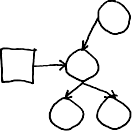
\includegraphics[width = \textwidth]{figures/expert-60-reduced.png}\\
                                  {\small     (a): hand drawing}
      \end{minipage}%
      \begin{minipage}[t]{\noisySize}
        \centering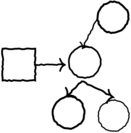
\includegraphics[width = \textwidth]{figures/60-1-reduced.png}\\
                                  {\small     (b): noisy render of (a)'s spec}
      \end{minipage}}%
    %% \visible<3->{\begin{minipage}{0.35\textwidth}
    %%     \begin{flushright}
    %%       \textbf{Learned distance metric}\\
    %%       \small    Serves as likelihood surrogate
    %%       \begin{align*}
    %%         \displaystyle\qquad    -\log L_{\text{learned}}(\text{render}&(S_1)|\text{render}(S_2))\approx\\& |S_1 - S_2| + |S_2 - S_1|
    %%       \end{align*}
    %%       $S_1$: noisy render\\
    %%       $S_2$: nonnoisy render
    %%     \end{flushright}
    %% \end{minipage}}%
    \hspace{0.2\textwidth}%
    \visible<3->{\begin{minipage}[c]{0.3\textwidth}
\vspace{-0.4cm}      \includegraphics[width = 0.8\textwidth]{figures/evaluationPhase1}
    \end{minipage}}
\end{frame}

\begin{frame}{Parsing images into \LaTeX~TikZ Commands}

  %% \vspace{-0.5cm}
{\footnotesize  Neurally Guided Procedural Modeling (Ritchie et al 2016) + Attend, Infer, Repeat (Eslami et al 2016)}
  \vspace{-0.5cm}
  \begin{center}
    \begin{tabular}{c}
\raisebox{-.5\height}{    \includegraphics[width = 0.6\textwidth]{architecture.pdf}            }
%%       &
%% \raisebox{-.5\height}{\includegraphics[width = 0.3\textwidth]{figures/averageNumberOfErrors.png}}
      \end{tabular}

  \end{center}
    \newcommand{\noisySize}{0.12\textwidth}
    \visible<1->{
\hspace{0.1\textwidth}      \begin{minipage}[t]{\noisySize}
        \centering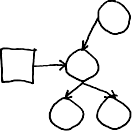
\includegraphics[width = \textwidth]{figures/expert-60-reduced.png}\\
                                  {\small     (a): hand drawing}
      \end{minipage}%
      \begin{minipage}[t]{\noisySize}
        \centering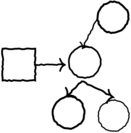
\includegraphics[width = \textwidth]{figures/60-1-reduced.png}\\
                                  {\small     (b): noisy render of (a)'s spec}
      \end{minipage}}%
    %% \visible<3->{\begin{minipage}{0.35\textwidth}
    %%     \begin{flushright}
    %%       \textbf{Learned distance metric}\\
    %%       \small    Serves as likelihood surrogate
    %%       \begin{align*}
    %%         \displaystyle\qquad    -\log L_{\text{learned}}(\text{render}&(S_1)|\text{render}(S_2))\approx\\& |S_1 - S_2| + |S_2 - S_1|
    %%       \end{align*}
    %%       $S_1$: noisy render\\
    %%       $S_2$: nonnoisy render
    %%     \end{flushright}
    %% \end{minipage}}%
    \hspace{0.2\textwidth}%
    \visible<1->{\begin{minipage}[c]{0.3\textwidth}
\vspace{-0.4cm}      \includegraphics[width = 0.8\textwidth]{figures/evaluationPhase2}
    \end{minipage}}
\end{frame}

\begin{frame}{Synthesizing high-level programs from specs (spec$ = $drawing commands)}
  Constraint-based program synthesis; SAT solver (Solar-Lezama 2008)
  \begin{equation*}
  %  \text{program}(S) = \argmin_{p\in \text{DSL, s.t. }p \text{ consistent w/ } S} \text{cost}(p)\label{programObjective}
    \text{program}(S) = \argmin_{\substack{p\in \text{DSL}\\p\text{ consistent w/ }S}} \text{cost}(p)
  \end{equation*}
  min cost$\approx$simple+short\\
  DSL: \textbf{D}omain \textbf{S}pecific \textbf{L}anguage: variables, arithmetic, loops, conditionals

  \vspace{0.8cm}

\footnotesize\centering    \begin{tabular}{rl}\toprule
  Program$\to$&Statement; $\cdots$; Statement\\
  Statement$\to$&\texttt{circle}(Expression,Expression)\\
  Statement$\to$&\texttt{rectangle}(Expression,Expression,Expression,Expression)\\
  Statement$\to$&\texttt{line}(Expression,Expression,Expression,Expression,Boolean,Boolean)\\
  Statement$\to$&\texttt{for}$(0\leq \text{Var}  < \text{Expression})$\texttt{ \{ if }$(\text{Var} > 0)$\texttt{ \{ }Program\texttt{ \}; }Program\texttt{ \}}\\
  Statement$\to$&\texttt{reflect}$(\text{Axis})$\texttt{ \{ }Program\texttt{ \}}\\
  Expression$\to$&$\mathbb{Z}\times$Var\texttt{+}$\mathbb{Z}$\\
%  Var$\to$&A free (unused) variable\\
  Axis$\to$&\texttt{X = }$\mathbb{Z}$ \vert \texttt{Y = }$\mathbb{Z}$\\
    $\mathbb{Z}\to$&an integer\\\bottomrule
  \end{tabular}

\end{frame}

\begin{frame}{Learning to quickly synthesize programs}
    Learn search policy $\pi (\text{program subspace} | \text{spec})$
  \\Think of the subspace as an ``ansatz''

OBJECTIVE (cf Bias-Optimal Search, Schmidhuber 2004):  $$\pi^* = \argmin_\pi\sum_{\text{spec}}\min_{\substack{\text{all subspaces}\\\text{subspace solves spec}}} \frac{\mathbb{E}[\text{time to exhaustively search the subspace}]}{\pi (\text{subspace}|\text{spec})}$$

  \vspace{-0.15cm}
    \begin{tikzpicture}[scale=0.8]
    \node[anchor = west] at (0,5.25) {Entire program search space};
\footnotesize    \draw[fill = yellow,fill opacity = 0.15,draw = black] (0,0) rectangle (5,5);
    \draw [fill = yellow, opacity = 0.2] (0,0)--(0,2)--(4,0)--(0,0);
    \draw [fill = yellow, opacity = 0.4] (0,5)--(0,1)--(3,5);
    \draw [fill = yellow, opacity = 0.6] (2.5,5)--(3.2,0)--(5,0)--(5,5);
    \draw (0,2) -- node[below,sloped]{short programs} (4,0);
    \draw (0,2) -- node[above,sloped]{long programs} (4,0);
    \draw (2.5,5) -- node[above,sloped]{programs w/ reflections} (3.2,0);
    \draw (0,1) -- node[above,sloped]{ programs w/ loops} (3,5);
    \node(p1)[anchor =west ] at (5.0,3.5) {$\pi(\text{short, no loop/reflect}|S) = $};
    \draw [fill = yellow, fill opacity = 0.2,draw = black]  ([xshift = 0cm,yshift = -0.2cm]p1.east) rectangle ([xshift = 0.4cm,yshift = 0.2cm]p1.east);
    \node(p2)[anchor =west ] at ([yshift = -0.5cm]p1.west) {$\pi(\text{long, loops}|S) = $};
    \draw [fill = yellow, fill opacity = 0.4,draw = black]  ([xshift = 0cm,yshift = -0.2cm]p2.east) rectangle ([xshift = 0.4cm,yshift = 0.2cm]p2.east);
    \node(p3)[anchor =west ] at ([yshift = -0.5cm]p2.west) {$\pi(\text{long, no loop/reflect}|S) = $};
    \draw [fill = yellow, fill opacity = 0.15,draw = black]  ([xshift = 0cm,yshift = -0.2cm]p3.east) rectangle ([xshift = 0.4cm,yshift = 0.2cm]p3.east);
    \node(p4)[anchor =west ] at ([yshift = -0.5cm]p3.west) {$\pi(\text{long, reflects}|S) = $};
    \draw [fill = yellow, fill opacity = 0.6,draw = black]  ([xshift = 0cm,yshift = -0.2cm]p4.east) rectangle ([xshift = 0.4cm,yshift = 0.2cm]p4.east);
    \node(p5)[anchor =west ] at ([yshift = -0.5cm]p4.west) {\emph{etc.}};
\visible<2->{        \node at (15.2,3) {\includegraphics[width = 3.6cm]{figures/2policyComparison}};}
  \end{tikzpicture}

\end{frame}

\begin{frame}{Application: Error correction}
  \textbf{learn prior over programs (simple$\approx$better), jointly infer likely parse+program}\\
  \textbf{Top-down influence upon perception}
  
  \vspace{0.4cm}
  
\def\arraystretch{0.0}
  \centering\begin{tabular}{p{3cm}p{3cm}p{3cm}}
\toprule     \centering Drawing&Neural net output&Corrected output\\\midrule 
\multicolumn{3}{c}{        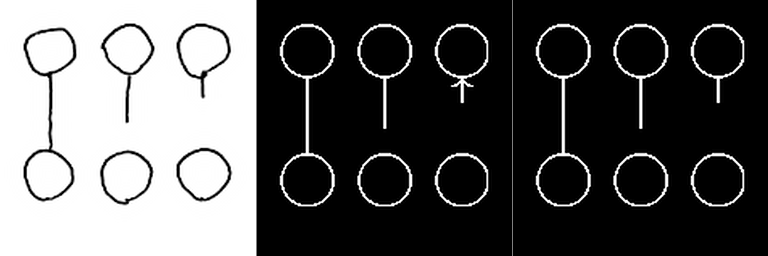
\includegraphics[width = 9cm]{figures/programSuccess7.png} }\\
\multicolumn{3}{c}{        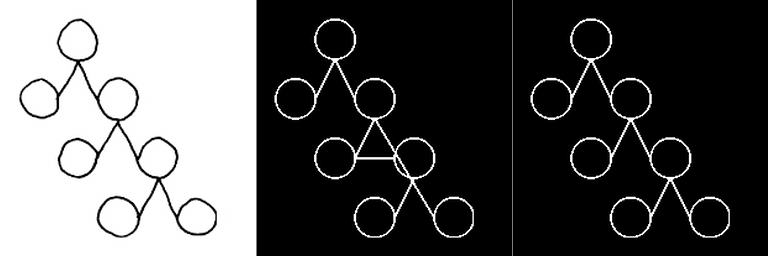
\includegraphics[width = 9cm]{figures/programSuccess16.png} }

    \end{tabular}

\end{frame}

\begin{frame}{Application: Extrapolating drawings}
  \centering  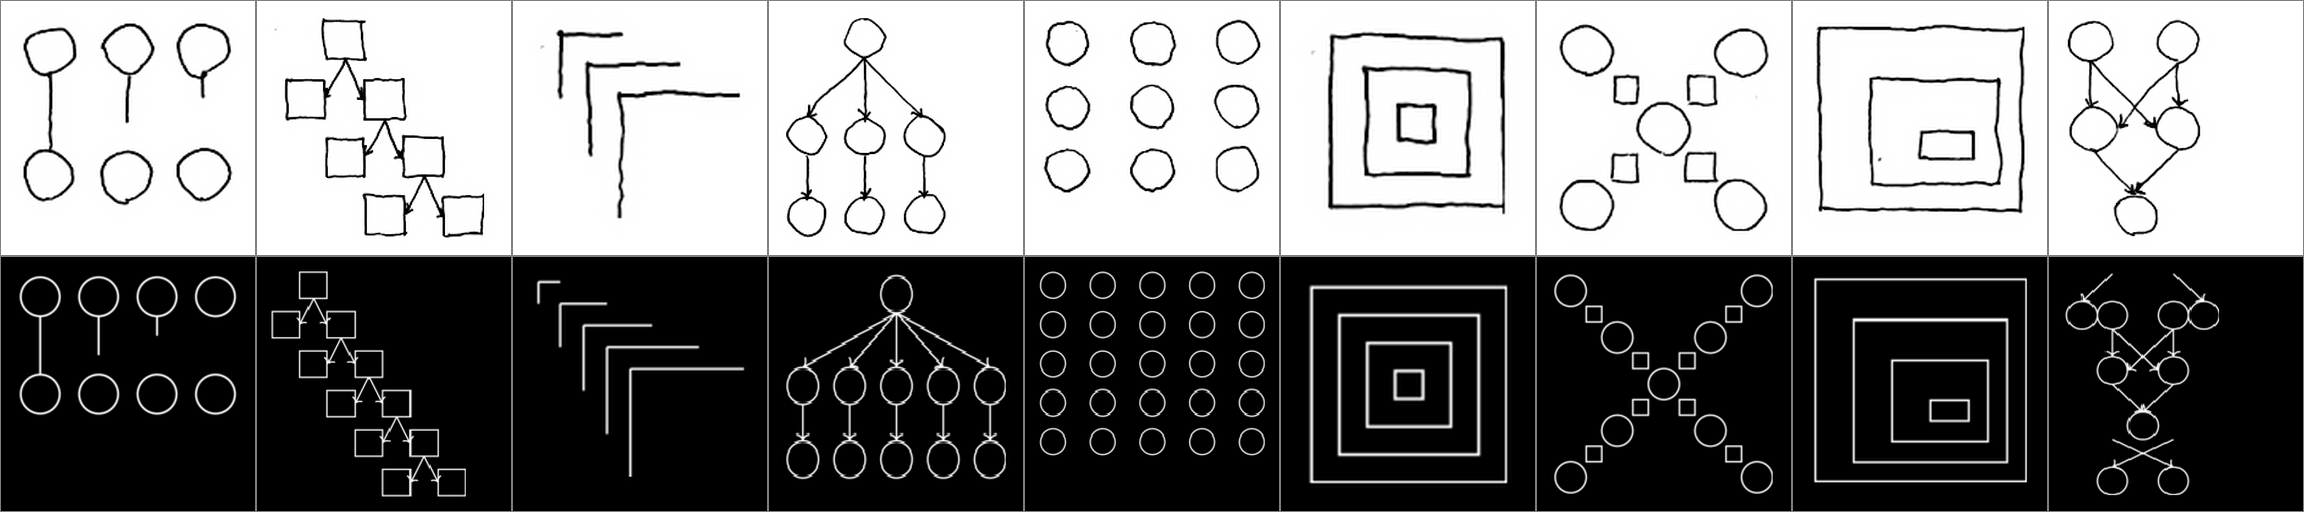
\includegraphics[height = 0.3\textheight]{figures/extrapolationMatrix1.png}
\\  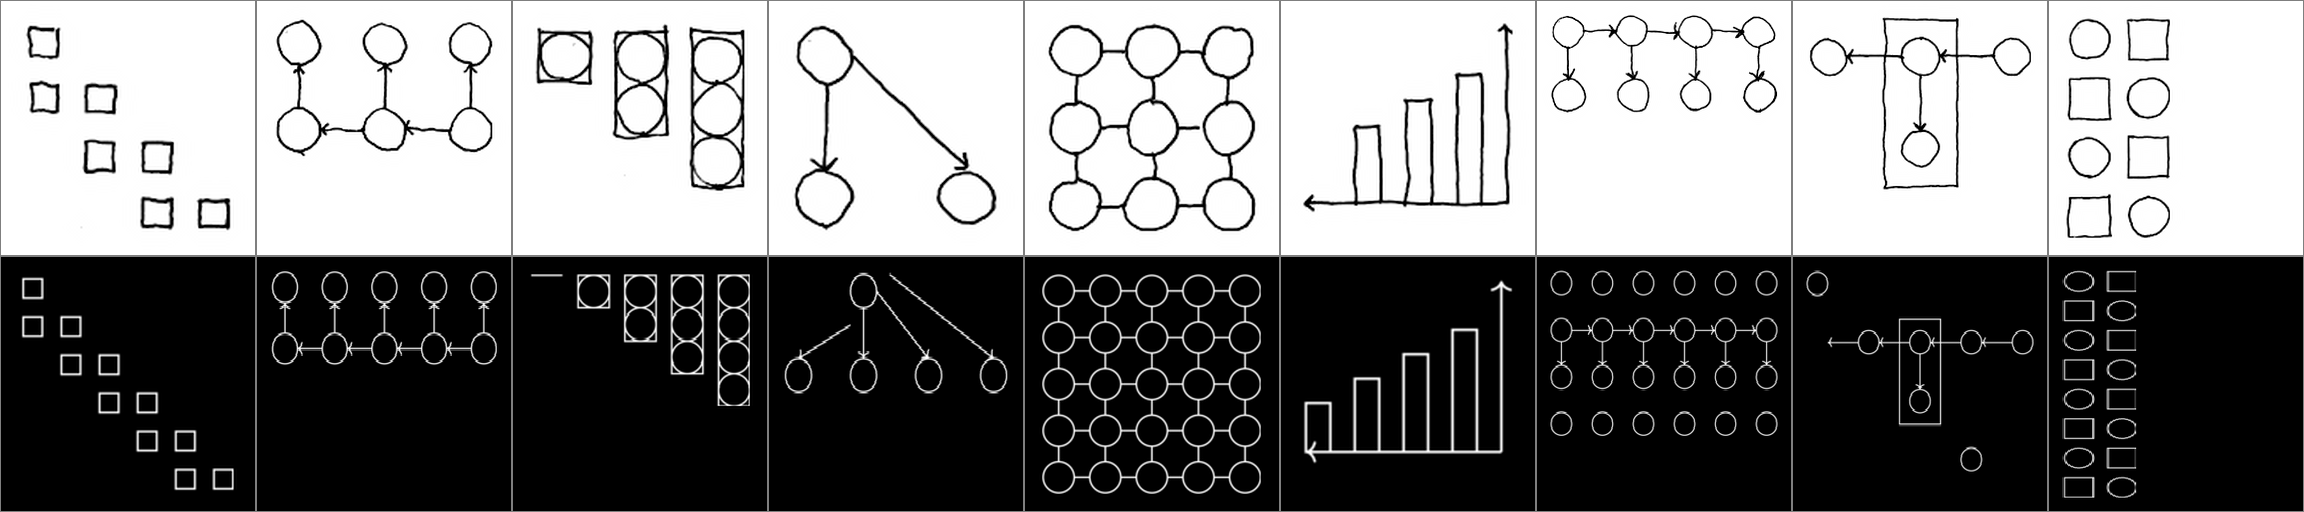
\includegraphics[height = 0.3\textheight]{figures/extrapolationMatrix2.png}
\\  \includegraphics[height = 0.3\textheight]{figures/extrapolationMatrix3.png}  


\end{frame}

\begin{frame}{\Huge Visual input$\to$Program: Poster AB \#25}

  \centering  \includegraphics[width = 0.8\textwidth]{firstSpotlightExample.pdf}
  \vspace{1cm}
\\\centering  \includegraphics[height = 0.3\textheight]{figures/extrapolationMatrix3.png}  

  \end{frame}

\end{document}

